%%%%%%%%%%%%%%%%%%%%%%%%%%%%%%%%%%%%%%%%%
% Thesis 
% LaTeX Template
% Version 1.3 (21/12/12)
%
% This template has been downloaded from:
% http://www.latextemplates.com
%
% Original authors:
% Steven Gunn 
% http://users.ecs.soton.ac.uk/srg/softwaretools/document/templates/
% and
% Sunil Patel
% http://www.sunilpatel.co.uk/thesis-template/
%
% License:
% CC BY-NC-SA 3.0 (http://creativecommons.org/licenses/by-nc-sa/3.0/)
%
% Note:
% Make sure to edit document variables in the Thesis.cls file
%
%%%%%%%%%%%%%%%%%%%%%%%%%%%%%%%%%%%%%%%%%

%----------------------------------------------------------------------------------------
%	PACKAGES AND OTHER DOCUMENT CONFIGURATIONS
%----------------------------------------------------------------------------------------

\documentclass[11pt, a4paper, oneside]{Thesis} % Paper size, default font size and one-sided paper

\usepackage{listings}
\lstset{language=C++, tabsize=2, breaklines=true, breakautoindent, postbreak=\raisebox{0ex}[0ex][0ex]{\ensuremath{\color{red}\hookrightarrow\space}}} 

\usepackage[square, numbers, comma, sort&compress]{natbib} % Use the natbib reference package - read up on this to edit the reference style; if you want text (e.g. Smith et al., 2012) for the in-text references (instead of numbers), remove 'numbers' 
\hypersetup{urlcolor=blue, colorlinks=true} % Colors hyperlinks in blue - change to black if annoying
\title{\ttitle} % Defines the thesis title - don't touch this
\usepackage{amsmath}
\usepackage{amsfonts}
\usepackage{amssymb}
\usepackage{amsthm}
\usepackage{todonotes}
\theoremstyle{definition}
\newtheorem{myexample}{Example}
\newtheorem{myremark}{Remark}
\newtheorem{mydef}{Definition}
\newtheorem{myproposition}{Proposition}
\newtheorem{myproof}{Proof}
\newtheorem{myobs}{Observation}

\begin{document}

\frontmatter % Use roman page numbering style (i, ii, iii, iv...) for the pre-content pages

\setstretch{1.3} % Line spacing of 1.3

% Define the page headers using the FancyHdr package and set up for one-sided printing
\fancyhead{} % Clears all page headers and footers
\rhead{\thepage} % Sets the right side header to show the page number
\lhead{} % Clears the left side page header

\pagestyle{fancy} % Finally, use the "fancy" page style to implement the FancyHdr headers

\newcommand{\HRule}{\rule{\linewidth}{0.5mm}} % New command to make the lines in the title page

% PDF meta-data
\hypersetup{pdftitle={\ttitle}}
\hypersetup{pdfsubject=\subjectname}
\hypersetup{pdfauthor=\authornames}
\hypersetup{pdfkeywords=\keywordnames}

%----------------------------------------------------------------------------------------
%	TITLE PAGE
%----------------------------------------------------------------------------------------

\begin{titlepage}
\begin{center}

\textsc{\LARGE \univname}\\[1.5cm] % University name
\textsc{\Large Extended Essay}\\[0.5cm] % Thesis type

\HRule \\[0.4cm] % Horizontal line
{\huge \bfseries \ttitle}\\[0.4cm] % Thesis title
\HRule \\[1.5cm] % Horizontal line
 
\begin{minipage}{0.4\textwidth}
\begin{flushleft} \large
\emph{Author:}\\
{\authornames} % Author name - remove the \href bracket to remove the link
\end{flushleft}
\end{minipage}
\begin{minipage}{0.4\textwidth}
\begin{flushright} \large
\emph{Supervisor:} \\
{\supname} % Supervisor name - remove the \href bracket to remove the link  
\end{flushright}
\end{minipage}\\[3cm]
 

 
{\large \today}\\[4cm] % Date
%\includegraphics{Logo} % University/department logo - uncomment to place it
 
\vfill
\end{center}

\end{titlepage}

%----------------------------------------------------------------------------------------
%	ABSTRACT PAGE
%----------------------------------------------------------------------------------------

\addtotoc{Abstract} % Add the "Abstract" page entry to the Contents

\abstract{\addtocontents{toc}{\vspace{1em}} % Add a gap in the Contents, for aesthetics
Many physical phenomena cannot be characterized by the idealizations of Euclidean geometry alone; they exhibit ``roughness'' of morphology. That is, they have a detailed structure at any arbitrarily small size scale. We can quantify this roughness with concepts of fractal dimension, which---just like the Euclidean dimension---tell how some figure fills a space. We explore the develpoment and utility of this concept, investigating three fractal dimensions: the similarity dimension and the box-counting dimension. We then describe the implementation of a computer algorithm to calculate the box-counting dimension of various fractals. Finally, we briefly examine the extension of fractal geometry to multifractal geometry.
}

\clearpage % Start a new page

%----------------------------------------------------------------------------------------
%	ACKNOWLEDGEMENTS
%----------------------------------------------------------------------------------------

\setstretch{1.3} % Reset the line-spacing to 1.3 for body text (if it has changed)

\acknowledgements{\addtocontents{toc}{\vspace{1em}} % Add a gap in the Contents, for aesthetics

I would like to thank my advisor, Ms. Langfield, for beating my first drafts into a bloody pulp and showing me how I could turn a disorganized mess into a piece of writing that I'm beginning to be proud of. I would also like to thank Prof. Tomasz Plewa and Tim Handy at the Department of Scientific Computing at Florida State University for giving me the impetus to study fractal and multifractal geometry and implement my knowledge computationally. 
}
\clearpage % Start a new page

%----------------------------------------------------------------------------------------
%	LIST OF CONTENTS/FIGURES/TABLES PAGES
%----------------------------------------------------------------------------------------

\pagestyle{fancy} % The page style headers have been "empty" all this time, now use the "fancy" headers as defined before to bring them back

\lhead{\emph{Contents}} % Set the left side page header to "Contents"
\tableofcontents % Write out the Table of Contents

\lhead{\emph{List of Figures}} % Set the left side page header to "List of Figures"
\listoffigures % Write out the List of Figures

\lhead{\emph{List of Tables}} % Set the left side page header to "List of Tables"
\listoftables % Write out the List of Tables.


%----------------------------------------------------------------------------------------
%	THESIS CONTENT - CHAPTERS
%----------------------------------------------------------------------------------------

\mainmatter % Begin numeric (1,2,3...) page numbering

\pagestyle{fancy} % Return the page headers back to the "fancy" style

% Include the chapters of the thesis as separate files from the Chapters folder
% Uncomment the lines as you write the chapters

% Chapter 1

\chapter{Fractals and their dimensions} % Main chapter title

\label{Chapter1} % For referencing the chapter elsewhere, use \ref{Chapter1} 

\lhead{Chapter 1. \emph{Fractal dimension}} % This is for the header on each page - perhaps a shortened title

%----------------------------------------------------------------------------------------

%----------------------------------------------------------------------------------------
\section{Why a fractal dimension is necessary}
We introduce two fractal shapes and observe various properties that lead them to be called fractals. We then show how characterizations of their geometry without fractal dimensions are not useful in differentiating one from another. 

\subsection{Example of a fractal: the Koch curve}\label{fractalexample}

We first discuss the Koch curve, one of the earliest fractals to be discovered. Shown in Fig. \ref{fig:kochcurve}, the curve was first constructed from a line segment by a recursive procedure \citep{Kochcurve}. However, it will be more useful to describe its construction in the following manner.

\begin{figure}[h]
\centering
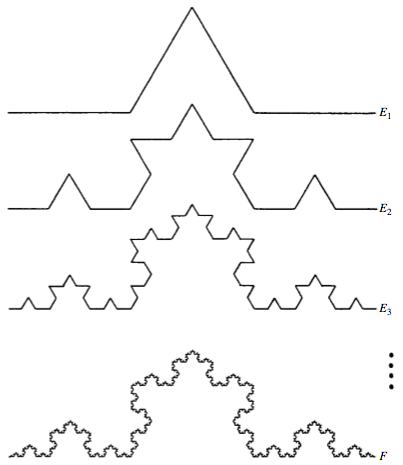
\includegraphics[height=0.6\textwidth]{Chapters/Figures/Kochcurve.png} 
\caption[Koch Curve]{Iterations of the Koch curve, a simple fractal exhibiting many characteristics typical of fractals. The initial figure at the top is made more and more textured with each iteration $E_{n}$, becoming rougher and more fractal-like as it approaches the final Koch curve $F$. Image credit: \citep{fractaltextbook}. }\label{fig:kochcurve}
\end{figure}

\paragraph{Construction of the Koch curve.} A curve $E_1$ is constructed by taking some line segment $E_0$ and dividing it into thirds. An equilateral triangle is constructed on the middle third of the segment $E_0$, such that the middle third of $E_0$ is one of the triangle's sides. The middle third of $E_0$ is then removed. Each successive iteration $E_n$ of the curve's generation is performed as follows: Each line segment in the $n$th iteration of the curve, having length $L_n$, is replaced by a scaled-down version of $E_1$ with length $4L_n/3$. 

The Koch curve $F$ is the result of an infinite number of applications of the iteration described above.
\begin{equation}\label{limitofE_n}
	F = \lim_{n \to \infty}E_n
\end{equation}

We note the most obvious properties of this fractal that separate it from a non-fractal shape. 

\begin{myobs}\textit{Its shape is defined recursively.} The Koch curve is a line segment on which an infinite number of the iterations described above is performed. This results in self-similarity at all scales: any section of the Koch curve contains an infinite number of repetitions of the original curve.\end{myobs}

\begin{myobs}\textit{The length of the Koch curve is infinite.}\end{myobs}

\begin{proof}
Because of the recursive rule defining the Koch curve, the curve's length is increased by a factor of $ 4/3 $ with each of the infinite iterations. We express the length of the curve after the $n$th iteration as $L_n$. 
\begin{equation}
	L_n = \left(\frac{4}{3}\right)^n L_0.
\end{equation}
The total length $L_\infty$ can be expressed as an infinite geometric sequence with a common ratio of $ 4/3 $:
\begin{equation}
	L_\infty = \lim_{n \to \infty}L_n = \lim_{n \to \infty}\left(\frac{4}{3}\right)^n L_0.
\end{equation}
Limits are linear with respect to multiplication by a constant, so we find:
\begin{equation}
	\lim_{n \to \infty}L_n = L_\infty = L_0 \lim_{n \to \infty} \left(\frac{4}{3}\right)^n,
\end{equation}
which clearly increases without bound.
\begin{equation}
	\lim_{n \to \infty}L_n = \infty 
\end{equation}
The length of the Koch curve is thus infinite.
\end{proof}

\begin{myobs}\textit{The Koch curve has no area.} Though we see that the additional length added with each iteration expands the fractal's size in the plane, the added segments have no thickness, so the area filled by the curve is thus zero.\end{myobs}


%---------------------------------
% CANTOR SET
%---------------------------------
\subsection{Another example of a fractal: the middle-third Cantor set}

We introduce a second fractal, the middle-third Cantor set, and show that it has drastically different properties from the Koch curve described above. It is shown in Fig. \ref{fig:cantorset} and was first described in \citep{Cantorset}.

\begin{figure}[h]
\centering
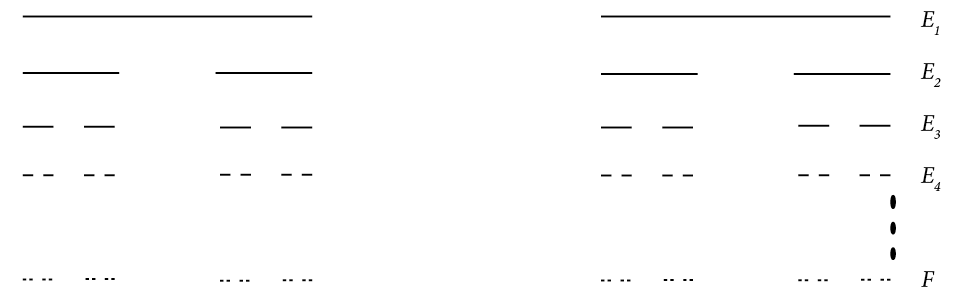
\includegraphics[width=0.9\textwidth]{Chapters/Figures/cantorset.png} 
\caption[Middle-third Cantor set]{Iterations of the middle-third Cantor set, another simple fractal. The initial figure at the top is made more and more sparse with each iteration $E_n$, before finally approaching the middle-third Cantor set, a figure that has no length, as we show below.}\label{fig:cantorset}
\end{figure}

\paragraph{Construction of the middle-third Cantor set.} 
A curve $E_1$ is constructed by taking some line segment $E_0$ and removing the middle third. Each successive iteration $E_n$ of the set's generation is performed by replacing each line segment in the $n$th iteration, having length $L_n$, with a scaled-down version of $E_1$ of length $L_n/3$. The middle-third Cantor set $F$ is the result of an infinite number of applications of the iteration described here, and is given by Eq. \ref{limitofE_n}.

We again note properties of this fractal that differentiate it from a non-fractal shape.

\begin{myobs}\textit{Its shape is defined recursively.} Just as with the Koch curve, this fractal is defined by a simple, recursive rule. This results in self-similarity at all scales: any portion of the set contains an infinite number of repetitions of the original set.\end{myobs}

\begin{myobs}\textit{Its length is zero.}\end{myobs}
\begin{proof}
We show that the length of the Cantor set is zero in the same way that we showed that the length of the Koch curve is infinite. 
Because of the recursive rule defining the Cantor set, the curve's length is decreased by a factor of $ 2/3 $ with each of the infinite iterations. We express the length of the curve after the $n$th iteration as $L_n$. 
\begin{equation}
	L_n = \left(\frac{2}{3}\right)^n L_0.
\end{equation}
The total length $L_\infty$ can be expressed as an infinite geometric sequence with a common ratio of $ 2/3 $:
\begin{equation}
	L_\infty = \lim_{n \to \infty}L_n = \lim_{n \to \infty}\left(\frac{2}{3}\right)^n L_0.
\end{equation}
As before,
\begin{equation}
	\lim_{n \to \infty}L_n = L_\infty = L_0 \lim_{n \to \infty} \left(\frac{2}{3}\right)^n
\end{equation}
which clearly tends toward zero.
\begin{equation}
	\lim_{n \to \infty}L_n = 0. 
\end{equation}
The length of the Cantor set is thus zero.
\end{proof}

\begin{myobs}\textit{Its area is zero.} The Cantor set consists of a line segment---something that has no thickness and thus fills no area---from which sections are removed. Because this process of removal does not add any thickness to the figure, the Cantor set must not have any thickness or area.\end{myobs}

\subsection{The ambiguity of nonfractal geometry}
We have now introduced two fractals. The first, the Koch curve, has infinite length but no area. The second, the middle-third Cantor set, has no length and no area. 

These characteristics do not, however, provide us much information about the fractals' shape: we can envisage many other fractals that, like the middle-third Cantor set, have neither length nor width but that also have entirely different appearances. In the middle-third Cantor set, we removed the middle $1/3$ of every line segment to generate the next iteration. Suppose instead that we construct a middle-fifteenth Cantor set. We perform an identical procedure to generate this fractal, but, instead of removing the middle third of each line segment, we remove the middle fifteenth. That is, we divide the line segment into fifteen equal parts and remove the middle one. The construction of such a set is depicted in Fig. \ref{fig:middle15}. 

\begin{figure}[h]
\centering
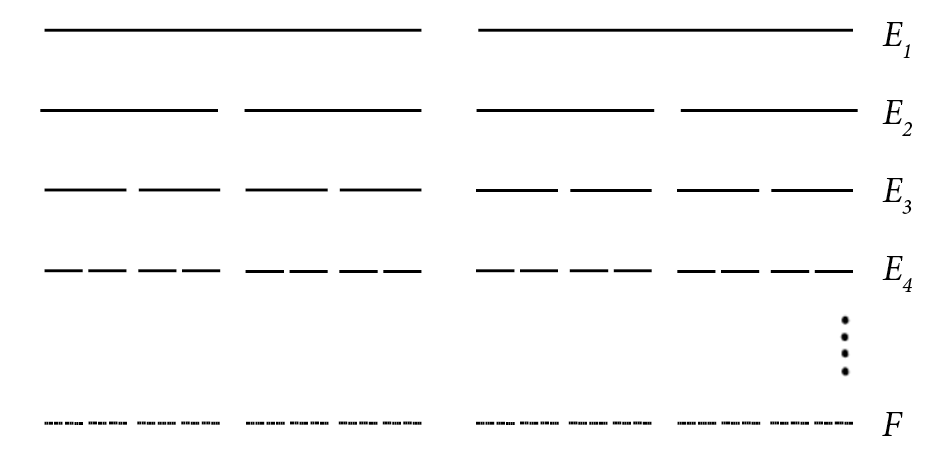
\includegraphics[width=0.9\textwidth]{Chapters/Figures/middle15.png} 
\caption[Middle-fifteenth Cantor set]{The middle-fifteenth Cantor set. This fractal is generated like middle-third Cantor set, except the middle fifteenth of each line segment is removed in every iteration. We see that the resulting fractal has a very different shape but show that it, like the middle-third Cantor set, has neither length nor area.}\label{fig:middle15}
\end{figure}

\begin{myobs}This middle-fifteenth Cantor set, though it has a different structure than the middle-third Cantor set, also has no length.\end{myobs}

\begin{proof}The length of the middle-fifteenth Cantor set can be expressed as an infinite geometric sequence, just as we did with the middle-third Cantor set. Here, though, the length is decreased by a factor of $14/15$ with each iteration, so the length $L_n$ of the set after $n$ iterations is given by
\begin{equation}
	L_n = \left(\frac{14}{15}\right)^n L_0.
\end{equation}
The final length of the curve $L_\infty$ is 
\begin{equation}
	L_\infty = \lim_{n \to \infty}L_n = \lim_{n \to \infty}\left(\frac{14}{15}\right)^n L_0,
\end{equation}
which still tends to zero as n tends toward infinity. Hence the length of the middle-fifteenth Cantor set is also zero.
\end{proof}

Instead of classifying fractals by their length and area, then, we examine their ``roughness''. This, as we will discuss below, leads to the creation of different \textit{fractal dimensions} to classify the space-filling properties of these fractals.

%---------------------------
% FRACTAL DIMENSIONS
%---------------------------
\section{What ``dimension'' means: an exploration of similarity dimension}
Consider a line segment of length $ L_0 $ and some number $\epsilon > 1$. Note that when the segment is scaled by $\epsilon$ into smaller pieces of equal size, each segment produced has length $L_0/\epsilon$. Now we repeat our exploration with a square of side length $ L_0 $. Here, when the square is scaled by a factor $\epsilon$, the smaller squares produced have an area $1/\epsilon^2$ the original. Again, when we repeat this procedure with a cube of side length $ L_0 $ we find that the cubes produced all have volumes $1/\epsilon^3$ the original. Hence, we generalize that the number of pieces $n$ produced from scaling by a factor of $\epsilon$ is given by 
\begin{equation}
n = 1/\epsilon^D
\end{equation}
where $D$ is the dimension of the shape, and we can now solve for dimension:
\begin{equation}\label{dimensionEqn}
 D = \frac{\log{n}}{\log{(1/\epsilon)}}
\end{equation}

\paragraph{Dimension of the Koch curve.} We now return to the Koch curve. We recognize the first iteration $E_1$ as the fundamental unit of all other iterations of the curve. That is, we can replace each of the four line segments that make up $E_1$ with a scaled-down copy of the original $E_1$ in order to reach the next iteration, and by repeating this process ad infinitum we can reach the final curve $F$. We can, however, view this process in the framework established in the example above, so that each iteration replaces one line segment with a length $L_0$ with four others, each of which has a length of $L_0/3$. This is akin to the method described above: our fractal produces $n = 4$ smaller pieces each time it is scaled, and each piece is $1/\epsilon = 1/3$ the size of the original. Hence, we can apply the equation for dimension (Equation \ref{dimensionEqn}) to the Koch curve:
\begin{equation}
D = \frac{\log{n}}{\log{(1/\epsilon)}} = \frac{\log{4}}{\log{3}} \approx 1.26
\end{equation}

\begin{myremark}What does this dimension mean? Again, it seems intuitive that the dimension would be between one and two. If the dimension were two or greater, the curve would completely fill the plane in which it lies. Likewise, if the dimension were one or less, the curve would 


---this generalization of dimension resembles the more familiar case of non-fractional dimensions. \end{myremark}

\section{Fractal dimensions}
In the previous section we introduced the concept of dimension to quantify how the size of a figure is related to its scaling factor. We found that a figure in two dimensions, for example, is scaled into four parts when scaled by a factor of two. This is only one of many ways that we can quantify the scaling of a shape. We must remember:

\begin{quote}
``There is no one dimension that can only describe a fractal set; many different types of dimension exist, and all provide very different conceptions of a fractal's properties'' \citep{fractaltextbook}.
\end{quote}

That is, dimension is just some quantity that describes the scaling relationship of a shape. We call the quantity described in the previous section the \emph{similarity dimension}. We will use the understanding we develop here to understand box-counting dimension and similarity dimension.

\subsection{Spaces, sets, and measures}
Before we venture further into classifying fractals by their dimension, we need the following definitions.

We use the word ``set'' to more precisely refer to what might be simply called a shape; every shape is just a set, possibly infinite, of points. As seen above, whereas non-fractal sets have well-defined, intuitively understood geometric properties such as length or area, fractal sets can be characterized by various concepts of dimension. Here, we will discuss \textit{box-counting dimension} in the greatest detail.



\begin{mydef}
An n-dimensional space $ \mathbb{R}^{n} $ is the set of all points that can be identified by an ordered n-ple of real numbers. Hence, for example, any point $ \alpha $ in $ \mathbb{R}^{5} $ can be identified by the ordered 5-ple $ \alpha = (\alpha_{1}, \alpha_{2}, \alpha_{3}, \alpha_{4}, \alpha_{5})$ where $ \alpha_{1} ... \alpha_{5} \in \mathbb{R} $.\end{mydef}

We will now work by analogy to discuss the concept of a \textit{measure}\footnote{Analogy adapted from \citep{mandelbrotmultifractal}}. Consider a geographical map of some landmass, with a function $ \mu(\mathcal{S}) $ that denotes the volume of groundwater below any subset $ \mathcal{S} $ of the landmass. We note four intuitive properties of this measure $ \mu $:\begin{enumerate}
\item The measure of any subset of the space---or the volume of groundwater under any plot of land on the landmass---gives a numerical indication of the plot of land's magnitude. That is, it describes the plot's size when measured by groundwater content.
\item\label{measureofanullset} There should be no water under a plot of land with no size. 
\item\label{measureofsubsets} If a plot of land $ A $ contains another plot of land $ B $, there should be less or as much groundwater under $B$ as there is under $A$. 
\item\label{measureaddition} If we find the volume of groundwater under a plot of land on the landmass, we should get the same value or less than when we split the plot up into many pieces with overlap allowed and add up the volume of groundwater found under each piece. 
\end{enumerate}
We now formalize these properties below.

\begin{mydef}
A measure $ \mu $ is a function on a space $ \mathbb{R}^{n} $ that assigns a positive number to each subset $ \mathcal{S} $ of $ \mathbb{R}^{n} $ such that:

\begin{itemize}
\item Because $\mu$ should characterize a set by its size in some sense, it is meaningless to have a nonzero size for any set with no elements. This is reflected in Property \ref{measureofanullset} above.
\begin{equation}
\mu(\emptyset) = 0
\end{equation}
\item The size of a set should be smaller than (or equal to, if $ A = B $, i.e., $B$ is not a proper subset of $A$) the size of a set that contains the first set and other elements too. This is reflected in Property \ref{measureofsubsets} above.
\begin{equation}
\mu(B) \le \mu(A) \mathrm{ \quad if \quad }  B \subset A.
\end{equation} 
\item The measure of a union of subsets should never be larger than the sum of the measures of the individual subsets: 
\begin{equation}
\mu\left(\bigcup_{i=1}^{\infty} A_i\right) \le \sum_{i=1}^{\infty} \mu(A_i) 
\end{equation}
Allowing for the measure of the union to be smaller than the sum of the individual measures accounts for overlap between the subsets; if, for all pairs of subsets $A_1$ and $A_2$, $A_1 \cap A_2 = \emptyset$, the measure of the union should be equal to the sum of the individual measures. In short, the measure should be distributive over addition. This is reflected in Property 4 above.
\end{itemize}

We call the space on which the measure resides the \textit{support} of the measure.
\end{mydef}

\subsection{Box-counting dimension}
Recall that in the example of the Koch curve above, we failed to usefully classify the shape by non-fractal means. Though we could see that the figure filled a space, we lacked language to discuss precisely how it filled that space; we could not quantify its ``roughness''. We introduce the box-counting dimension as an analogy to the Euclidean dimension in order to quantify how a fractal set fills a space.

We now seek to formalize our understanding of dimension. Furthermore, we wish to formalize this understanding in a way that allows us to discuss fractal objects that are not strictly self-similar\footnote{Fractals are not as concretely defined as one might hope. We tend only to classify a shape as a fractal when it possesses a reasonably large number of the fractal properties identified in Sec 1.1---when a shape has sufficient ``roughness'' that the language of fractal geometry becomes more useful in describing its characteristics.}. For this we introduce a specific dimension, the \textit{box-counting dimension}. In addition, the box-counting dimension is computationally much more simple than other fractal dimensions, such as the Hausdorff dimension \citep{fractaltextbook}.

The box-counting dimension gives an analogue of the dimension defined by Equation \ref{dimensionEqn}: the fractal set is covered by a number of cubes\footnote{A ``cube'' here is not strictly three-dimensional; the shape has analogues in all other dimensions as well. A cube in $\mathbb{R}^n$ is more generally a figure with $2n$ sides of equal size where each side is orthogonal to the others it touches, if the others exist, and each side is itself a cube in $\mathbb{R}^{n-1}$. Thus a cube in $\mathbb{R}^1$ is a line segment; a cube in $\mathbb{R}^2$ is a square; and a cube in $\mathbb{R}^4$ is a tesseract.} with side length $\epsilon$. We extend the number of replacements $ n $ from Equation \ref{dimensionEqn} to take the smallest number of cubes that can cover the fractal set. The box-counting dimension is given by the limit of this extension of Equation \ref{dimensionEqn} as the side $\epsilon$ approaches zero.

\begin{mydef} The box-counting dimension of a fractal set $ F $, $\operatorname{dim}_B F $, is given by:
\begin{equation}\label{boxcountingeqn}\operatorname{dim}_B F = \lim_{\epsilon \to 0} \frac{\log N_\epsilon(F)}{-\log\epsilon}
\end{equation}
where $N_\epsilon(F)$ is the number of cubes of side-length $\epsilon$ that cover the fractal set $F$.
\end{mydef}

It is simple, computationally, to discretize the cubes---or, boxes---that cover the fractal set. In addition, it is simple to implement an algorithm that evaluates the limit in Eq. \ref{boxcountingeqn} by assessing which boxes do or do not cover the fractal set. A computational implementation of a box-counting algorithm is described in the following chapter. We use this implementation to examine the relationship between the box-counting and theoretical dimensions of the Koch curve.































% Chapter Template

\chapter{Applications} % Main chapter title

\label{Chapter2} % Change X to a consecutive number; for referencing this chapter elsewhere, use \ref{ChapterX}

\lhead{Chapter 2. \emph{Applications}} % Change X to a consecutive number; this is for the header on each page - perhaps a shortened title



 
% Chapter Template

\chapter{Applications} % Main chapter title

\label{Chapter3} % Change X to a consecutive number; for referencing this chapter elsewhere, use \ref{ChapterX}

\lhead{Chapter 3. \emph{Applications}} % Change X to a consecutive number; this is for the header on each page - perhaps a shortened title

%----------------------------------------------------------------------------------------
%	SECTION 1
%----------------------------------------------------------------------------------------


%\input{./Chapters/Chapter4} 
%\input{./Chapters/Chapter5} 
%\input{./Chapters/Chapter6} 
%\input{./Chapters/Chapter7} 

%----------------------------------------------------------------------------------------
%	THESIS CONTENT - APPENDICES
%----------------------------------------------------------------------------------------

\addtocontents{toc}{\vspace{2em}} % Add a gap in the Contents, for aesthetics

\appendix % Cue to tell LaTeX that the following 'chapters' are Appendices

% Include the appendices of the thesis as separate files from the Appendices folder
% Uncomment the lines as you write the Appendices

% Appendix A
\chapter{Source Code of Box-Counting Module} % Main appendix title
\usepackage{listings}
\lstset{language=C++} 
\label{AppendixA} % For referencing this appendix elsewhere, use \ref{AppendixA}

\lhead{Appendix A. \emph{Box-Counting Module}} % This is for the header on each page - perhaps a shortened title

\begin{lstlisting}
/** Fractal analysis module utilizing boxcounting to determine 
	the fractal dimension of a shape in the input text/binary file.

	Prints to terminal:
		- the results at each level of analysis
		- the overall dimension as determined by least-squares regression
		- an R^2 value
		
	@author Samuel Brenner
	@version July 11, 2013

**/



#include <fstream>
#include <string>
#include <sstream>
#include <math.h>
#include <iostream>
#include "regressionModule.h"
#include "dataReader.h"
#include "interpolation.h"

using namespace std;

const char* fileName = "c_hdf5_plt_cnt_1000.txt";
//const char* fileName = "first(phillip's).txt";

const char* outFileName = "logN-vs-logE.txt";


void printArray(int** arrayIn, int HEIGHT, int WIDTH){
	cout << endl;
	for(int i = 0; i < HEIGHT; i++){
		for(int j = 0; j < WIDTH; j++){
			printf("%3d", arrayIn[i][j]);
		}
		printf("\n");
	 }
}

void printArray(double** arrayIn, double HEIGHT, double WIDTH){
	cout << endl;
	printf("%7s%7s\n", "level", "log(n)");
 	for(int i = 0; i < HEIGHT; i++){
		for(int j = 0; j < WIDTH; j++){
			printf("%7.3f ", arrayIn[i][j]);
		}
		printf("\n");
 	}
}

void printToFile(double** arrayIn, int HEIGHT, int WIDTH, double slope, double yint){
	FILE * pFile;
	pFile = fopen(outFileName, "w");
	fprintf(pFile, "slope: %f\nintercept: %f\n", slope, yint);
	for(int i = HEIGHT - 1; i >= 0; i--){
		for(int j = 0; j < WIDTH; j++){
			fprintf(pFile, "%-2.6f ", arrayIn[i][j]);
		}
		fprintf(pFile, "\n");
	}
	fclose(pFile);
}

/**
	Returns the log base 2 of the number of cells filled in a given level
	of fractal analysis.
	@param arrayIn is the 2-3-D array of integers that contains the data
	@param HEIGHT
	@param WIDTH
	@param DPETH
	@param level is the level of analysis to be performed. Level 0, for example, 
	examines only the individual data points, whereas at level 1 they are merged
	into boxes of side length 2^1, and for level l size 2^l.
	@return log base 2 of the number of cells filled in a given level.

**/
double boxCounting(int*** arrayIn, int HEIGHT, int WIDTH, int DEPTH, int level){
	int numberFilled = 0; //number of boxes with an element of the figure
	int boxDimension = (int) pow(2, level);
	int boxDimensionZ;

	if(DEPTH != 1){
		boxDimensionZ = boxDimension;
	}
	else{
		boxDimensionZ = 1;
	}
	//iterates through all boxes
	//cout << "here!" << endl;
	for(int i = 0; i < HEIGHT; i += boxDimension){
		for(int j = 0; j < WIDTH; j += boxDimension){
			for(int k = 0; k < DEPTH; k += boxDimensionZ){
				int boxSum = 0;


				//sums each box
				for(int boxSumX = 0; boxSumX < boxDimension; boxSumX++){
					for(int boxSumY = 0; boxSumY < boxDimension; boxSumY++){
						for(int boxSumZ = 0; boxSumZ < boxDimensionZ; boxSumZ++){
							//if(boxSumX + i >= HEIGHT || boxSumY + j >= WIDTH || boxSumZ + k >= DEPTH){ This is to deal with dimensions that aren't
							//	cout << endl << "Dimensions must be powers of two!" << endl;				powers of two.
							//	boxSum += 0;
							//}
							//else{
								boxSum += arrayIn[boxSumX + i][boxSumY + j][boxSumZ + k];
							//}
						}
					}
				}

				if(boxSum > 0){
					numberFilled++;
				}

			}
		}
	}
	printf("%s%d\n%s%d\n%s%d\n\n", "level: ", level, 
	"--box dimension: ", boxDimension, "--filled boxes: ", numberFilled);		

	return log2(numberFilled);
}

int main () {
	int HEIGHT, WIDTH, DEPTH;
	double*** elements;
	bool haveZeros = false;
	double arraySum;
	int*** elementsInterpolated;

	elements = dataReaderASCII<double>(fileName, HEIGHT, WIDTH, DEPTH, haveZeros, arraySum); //change to dataReaderASCII to read in text files
	elementsInterpolated = interpolate(elements, HEIGHT, WIDTH, DEPTH, 0.5);
	//printToFile(elementsInterpolated, HEIGHT, WIDTH);

	int LOWESTLEVEL = 0;

	//initialize out-array
	int largestDimension = fmin(HEIGHT, WIDTH);
	if(DEPTH > 1){
		largestDimension = fmin(largestDimension, DEPTH);
	}
	int outArrayLength = int(log2(largestDimension) - LOWESTLEVEL + 1);
	double** outDataArray = new double* [outArrayLength];

	//printf("\n\n%d\n\n", outArrayLength);

	for(int i = 0; i < outArrayLength; i++){
		outDataArray[i] = new double[2];
	}

	for(int k = 0; k < outArrayLength; k++)
	{
		outDataArray[k][0] = outArrayLength - 1 - (k + LOWESTLEVEL);
		outDataArray[k][1] = boxCounting(elementsInterpolated, HEIGHT, WIDTH, DEPTH, k + LOWESTLEVEL);
	}

	printArray(outDataArray, outArrayLength, 2);

	double* regressionArray = new double[3];

	slope(outDataArray, outArrayLength, regressionArray);

	printf("\n\n%s%s\n\n%s%.5f\n%s%1.3f\n\n", "Curve: ", fileName, "Dimension: ", regressionArray[0], "R^2: ", regressionArray[1]);

	printToFile(outDataArray, outArrayLength, 2, regressionArray[0], regressionArray[2]);

	delete[] elements;
	delete[] elementsInterpolated;
	delete[] outDataArray;
	delete[] regressionArray;

	return 0;
}

/**
	Module to interpolate the isocontour at some pre-specified value inside a 2- or 3-D array.

	Implemented in boxCounter3D.cpp:
		Fractal analysis module utilizing boxcounting to determine 
		the fractal dimension of a shape in the input text/binary file.

		Prints to terminal:
			- the results at each level of analysis
			- the overall dimension as determined by least-squares regression
			- an R^2 value
			
		@author Samuel Brenner
		@version July 11, 2013

	@author Samuel Brenner
	@version July 11, 2013

**/

#ifndef interpolation_h
#define interpolation_h

int*** interpolate(double*** arrayIn, int HEIGHT, int WIDTH, int DEPTH, double valueToFind){
	//Declare and initialize arrayOut. If any values in the arrayIn happen to be the valueToFind,
	//we'll initialize the corresponding arrayOut to a 1; otherwise it'll be a 0.
	int*** arrayOut = new int**[HEIGHT];
	for(int i = 0; i < HEIGHT; i++){
		arrayOut[i] = new int*[WIDTH];
		for(int j = 0; j < WIDTH; j++){
			arrayOut[i][j] = new int[DEPTH];
			for(int k = 0; k < DEPTH; k++){
				//performs a preliminary check so that we don't miss any values that are exactly == valueToFind
				if(arrayIn[i][j][k] == valueToFind){
					arrayOut[i][j][k] = 1;
				}
				else{
					arrayOut[i][j][k] = 0;
				}
			}
		}
	}

	//Makes the interpolater able to handle planar data
	int startingDepthIndex = 0;
	if(DEPTH != 1){
		startingDepthIndex = 1;
	}
	else{
		DEPTH++;
	}

	/*
		Iterates over all entries in the array that aren't on the edge of the array, unless the array is 2D: for 2D
		arrays the program ignores the edge condition in the third dimension.

		For each entry analyzed, we check to see if the value is lower than valueToFind. If so, the neighbors on all 
		six sides (four if planar data) are checked against it to determine if there is some crossing over valueToFind
		in between the two. Then we determine which cell should contain that crossing and assign it a 1 in the 
		corresponding cell of the outArray.
	*/
	for(int i = 1; i < HEIGHT - 1; i++){
		for(int j = 1; j < WIDTH -1; j++){
			for(int k = startingDepthIndex; k < DEPTH - 1; k++){
				if(arrayIn[i][j][k] < valueToFind){
					if(arrayIn[i + 1][j][k] > valueToFind){
						if(int((valueToFind - arrayIn[i][j][k]) / (arrayIn[i + 1][j][k] - arrayIn[i][j][k])) == 0){
							arrayOut[i][j][k] = 1;
						}
						else{
							arrayOut[i + 1][j][k] = 1;
						}
					}
					if(arrayIn[i][j + 1][k] > valueToFind){
						if(int((valueToFind - arrayIn[i][j][k]) / (arrayIn[i][j + 1][k] - arrayIn[i][j][k])) == 0){
							arrayOut[i][j][k] = 1;
						}
						else{
							arrayOut[i][j + 1][k] = 1;
						}
					}
					if(arrayIn[i][j - 1][k] > valueToFind){
						if(int((valueToFind - arrayIn[i][j][k]) / (arrayIn[i][j - 1][k] - arrayIn[i][j][k])) == 0){
							arrayOut[i][j][k] = 1;
						}
						else{
							arrayOut[i][j - 1][k] = 1;
						}
					}
					if(arrayIn[i - 1][j][k] > valueToFind){
						if(int((valueToFind - arrayIn[i][j][k]) / (arrayIn[i - 1][j][k] - arrayIn[i][j][k])) == 0){
							arrayOut[i][j][k] = 1;
						}
						else{
							arrayOut[i - 1][j][k] = 1;
						}
					}
					if(arrayIn[i][j][k + 1] > valueToFind){
						if(int((valueToFind - arrayIn[i][j][k]) / (arrayIn[i][j][k + 1] - arrayIn[i][j][k])) == 0){
							arrayOut[i][j][k] = 1;
						}
						else{
							arrayOut[i][j][k + 1] = 1;
						}
					}
					if(arrayIn[i][j][k - 1] > valueToFind){
						if(int((valueToFind - arrayIn[i][j][k]) / (arrayIn[i][j][k - 1] - arrayIn[i][j][k])) == 0){
							arrayOut[i][j][k] = 1;
						}
						else{
							arrayOut[i][j][k - 1] = 1;
						}
					}

				}
			}
		}
	}

return arrayOut;
}

#endif

/**
	Module to run regression for boxcounting.
	
	Changes a double[3] such that regressionArray[0] = slope,
	regressionArray[1] = R^2, and regressionArray[2] = y-int.

	Implemented in boxCounter3D.cpp:
		Fractal analysis module utilizing boxcounting to determine 
		the fractal dimension of a shape in the input text/binary file.

		Prints to terminal:
			- the results at each level of analysis
			- the overall dimension as determined by least-squares regression
			- an R^2 value
			
		@author Samuel Brenner
		@version July 11, 2013

	@author Samuel Brenner
	@version July 11, 2013

**/


#include "regressionModule.h"

#include <math.h>

double stdev(double* arrayIn, double arrayMean, int arrayLength);

double corrCoeff(double* arrayX, double* arrayY, double meanX, 
	double meanY, double stdevX, double stdevY, int length);

double mean(double* arrayIn, int arrayLength);

void slope(double** arrayIn, int arrayLength, double* regressionArray){
	
	double* arrayX = new double[3];

	for(int i = 0; i < 3; i++){
		arrayX[i] = arrayIn[i][0];
	}

	double* arrayY = new double[3];
	for(int i = 0; i < 3; i++){
		arrayY[i] = arrayIn[i][1];
	}

	double meanX = mean(arrayX, 3);
	double meanY = mean(arrayY, 3);

	double stdevX = stdev(arrayX, meanX, 3);
	double stdevY = stdev(arrayY, meanY, 3);

	double r = corrCoeff(arrayX, arrayY, meanX, meanY, stdevX, stdevY, 3);

	double slope = r 
		* stdevY / stdevX;


	delete[] arrayX;
 	delete[] arrayY;

 	regressionArray[0] = slope;
 	regressionArray[1] = pow(r, 2);
 	regressionArray[2] = meanY - slope * meanX;
}

double stdev(double* arrayIn, double arrayMean, int arrayLength){

	double squaresSum = 0;

	for(int i = 0; i < arrayLength; i++){
		squaresSum += pow(arrayIn[i] - arrayMean, 2);
	}

	return sqrt(squaresSum / (arrayLength - 1));
}

double corrCoeff(double* arrayX, double* arrayY, double meanX, 
	double meanY, double stdevX, double stdevY, int length){

	double sum = 0;

	for(int i = 0; i < length; i++){
		sum += (arrayX[i] - meanX) * (arrayY[i] - meanY);
	}

	return sum / (stdevX * stdevY * (length - 1));
}

double mean(double* arrayIn, int arrayLength){
	double sum = 0;

	for(int i = 0; i < arrayLength; i++){
		sum += arrayIn[i];
	}

	return sum / arrayLength;
}

\end{lstlisting}
% Appendix Template

\chapter{Source Code of Multifractal Spectrum Module} % Main appendix title
\label{AppendixB} % For referencing this appendix elsewhere, use \ref{AppendixA}
\lstset{language=C++} 


\lhead{Appendix B. \emph{Multifractal Spectrum Module}} % This is for the header on each page - perhaps a shortened title

\begin{lstlisting}

/** 
	Multifractal analysis module utilizing boxcounting to determine 
	the multifractal spectrum of a measure in the input text/binary file.

	Prints the data that forms the multifractal spectrum to a text file
	that can later be analyzed in Matlab or another visualization program.

	The algorithm used is described in:
		A. Chhabra and R. V. Jensen, Phys. Rev. Lett. 62, 1330 (1989).

	@author Samuel Brenner
	@version July 11, 2013
**/
#include <fstream>
#include <string>
#include <sstream>
#include <math.h>
#include <iostream>
#include <algorithm>
#include "dataReader.h"
#include "dataCorrection.h"


using namespace std;


const char* fileName = "multifractal.txt"; //filename of input data--can also be binary

double qMin = -10;	//minimum and maximum values of the moment used in 
double qMax = 10;
double qIncrement = 1.0; //the step used between each value of q tested.

void printArray(int** arrayIn, int HEIGHT, int WIDTH){
	cout << endl;
	for(int i = 0; i < HEIGHT; i++){
		for(int j = 0; j < WIDTH; j++){
			printf("%7d", arrayIn[i][j]);
		}
		printf("\n");
	 }
}

void printArray(double** arrayIn, int arrayHeight, int WIDTH){
	cout << endl;
 	for(int i = 0; i < arrayHeight; i++){
		for(int j = 0; j < WIDTH; j++){
			printf("%3.3f ", arrayIn[i][j]);
		}
		printf("\n");
 	}
}

void printToFile(double** arrayIn, int level, int HEIGHT){
	FILE * pFile;
	char* fileOutName = new char[20];
	sprintf(fileOutName, "%s%d%s", "falphaout/falpha_level_", level, ".txt");
	pFile = fopen(fileOutName, "w");
	for(int i = 0; i < HEIGHT; i++){
		fprintf(pFile, "%.8f %.8f", arrayIn[i][0], arrayIn[i][1]);
		fprintf(pFile, "\n");
	}
	fclose(pFile);
	delete[] fileOutName;
}

/**	
	Returns in a double** the data points that make up the plot of f(alpha) vs. alpha.
	The analysis is performed using the method of moments described in Chhabra and Jensen, 
	1989 (Phys. Rev. Lett.).
	@param arrayIn is the 2-/3-D array of doubles that contains the data
	@param HEIGHT
	@param WIDTH
	@param DPETH
	@param level is the level of analysis to be performed. Level 0, for example, 
	examines only the individual data points, whereas at level 1 they are merged
	into boxes of side length 2^1, and for level l size 2^l.
	@return alpha vs. f(alpha)
**/
double** boxCounting(double*** arrayIn, int HEIGHT, int WIDTH, int DEPTH, int level){
	int boxDimension = (int) pow(2, level); //side length of the boxes that we'll use to coarse-grain the data, in pixels.
	int boxDimensionZ;

	if(DEPTH != 1){
		boxDimensionZ = boxDimension;
	}
	else{
		boxDimensionZ = 1;
	}

	int nDataPts = HEIGHT * WIDTH * DEPTH / pow(boxDimension, 2) / boxDimensionZ;
	int falphaSize = qMax - qMin + 1;

	//creates array to hold falpha
	double** falpha = new double*[falphaSize];
	for(int i = 0; i < qMax - qMin + 1; i++){
		falpha[i] = new double[2];
	}

	/**	iterates over all values of q to be tested, where q is the "microscope for exploring different regions of the measure",
		an exaggerating exponent that gives us the qth moment of the measure. We parametrize the relationship f(alpha) vs. alpha
		in terms of q to find functions f(q) and alpha(q). These values are then added to the falpha out-array.
	**/
	for(double q = qMin; q <= qMax; q += qIncrement){
		double* probability = new double[nDataPts]; //an array of all the non-normalized measures taken in.
		double sumOfProbabilitiesQthMoment = 0.0;
		int arrayCounter = 0;
		double fOfQ = 0.0;
		double alphaOfQ = 0.0;

		//iterates through all boxes
		for(int i = 0; i < HEIGHT; i += boxDimension){
			for(int j = 0; j < WIDTH; j += boxDimension){
				for(int k = 0; k < DEPTH; k += boxDimensionZ){
					double boxSum = 0.0;

					//sums each box
					for(int boxSumX = 0; boxSumX < boxDimension; boxSumX++){
						for(int boxSumY = 0; boxSumY < boxDimension; boxSumY++){
							for(int boxSumZ = 0; boxSumZ < boxDimensionZ; boxSumZ++){
								
								//This is to deal with dimensions that aren't powers of two.
									//if(boxSumX + i >= HEIGHT || boxSumY + j >= WIDTH || boxSumZ + k >= DEPTH){ 
									//	cout << endl << "Dimensions must be powers of two!" << endl;				
									//	boxSum += 0;
									//}
									//else{
									boxSum += arrayIn[boxSumX + i][boxSumY + j][boxSumZ + k];
									//}
							}
						}
					}
					probability[arrayCounter] = boxSum;
					arrayCounter++;
				}
			}
		}
	
		for(int i = 0; i < nDataPts; i++){
			sumOfProbabilitiesQthMoment += pow(probability[i], q); //the denominator in eqn. 6 of Chhabra and Jensen
		}

		double log2size = log2(double(boxDimension) / HEIGHT);

		for(int i = 0; i < nDataPts; i++){
			double normalizedMeasure = pow(probability[i], q) / sumOfProbabilitiesQthMoment; //eqn. 6 of Chhabra and Jensen
			//cout << log2(normalizedMeasure) << endl;
			fOfQ += normalizedMeasure * log2(normalizedMeasure); //the numerator of eqn. 7 of Chhabra and Jensen
			alphaOfQ += normalizedMeasure * log2(probability[i]); //the numerator of eqn. 8 of Chhabra and Jensen
		}

		falpha[int(q - qMin)][0] = alphaOfQ / log2size; //the final divisions in each equation
		falpha[int(q - qMin)][1] = fOfQ / log2size;
		delete[] probability;
	}

	return falpha;
}

int main () {
    int HEIGHT, WIDTH, DEPTH;
    double*** elements;
    bool haveZeros = false;
    double arraySum;

    elements = dataReaderASCII<double>(fileName, HEIGHT, WIDTH, DEPTH, haveZeros, arraySum); 
    //elements = dataReaderBinary<double>(fileName, HEIGHT, WIDTH, DEPTH, haveZeros, arraySum); //for reading in binary data

    /**	
    	Corrects the data by removing zeros (does so by adding one to every value in the array)
    	and normalizing the array so that the sum of all the elements is one.
    **/
    dataCorrection<double>(elements, HEIGHT, WIDTH, DEPTH, haveZeros, arraySum);

	int LOWESTLEVEL = 0; 	//the lowest level of coarse-graining, where level == 0 examines each individual pixel as its own box.
							//level = log2(box's side length) so that side length = 1 when level == 0.

	//iterates over all levels to be tested, going from LOWESTLEVEL to the highest possible level permitted by the arrayIn size.
	for(int k = 0; k < log2(HEIGHT) - LOWESTLEVEL; k++){
		cout << endl << "Level: " << k + LOWESTLEVEL << endl;
		double** falpha = boxCounting(elements, HEIGHT, WIDTH, DEPTH, k + LOWESTLEVEL);
		printArray(falpha, qMax - qMin + 1, 2);
		printToFile(falpha, k + LOWESTLEVEL, qMax - qMin + 1); //This spectrum output can then be analyzed in Matlab or another visualization program.
	}

	
	//delete[] buffer;
	delete[] elements;
	return 0;
}


\end{lstlisting}
% Appendix Template

\chapter{Source Code of Iterative Function System Generator} % Main appendix title
\label{AppendixC} % For referencing this appendix elsewhere, use \ref{AppendixA}
\lstset{language=C++} 


\lhead{Appendix C. \emph{IFS Generator}} % This is for the header on each page - perhaps a shortened title

\begin{lstlisting}
//Program to generate fractals in text.
#include <fstream>
#include <string>
#include <sstream>
#include <math.h>
#include <iostream>

using namespace std;

int HEIGHT = pow(2, 9);
int WIDTH = HEIGHT;
//double normalizer = 1;//double(pow(5.0, log2(HEIGHT)));

struct point{
	double probability;
	int value; 
};

void assignProbabilities(point** fractalArray){
	double fractalSum = 0.0;
	for(int levelDivision = HEIGHT; levelDivision > 1; levelDivision /= 2){
		for(int i = 0; i < HEIGHT; i++){
			for(int j = 0; j < WIDTH; j++){

				if((i % levelDivision >= (levelDivision / 2)) && (j % levelDivision >= (levelDivision / 2))){
					fractalArray[i][j].probability *= 2.0 / 5.0;
				}
				else{
					fractalArray[i][j].probability *= 1.0 / 5.0;
				}

				fractalSum += fractalArray[i][j].probability;

			}
		}
	}
	double fractalSumNew = 0.0;

	//divide each element by a certain factor so that the total probability is still one.
	
	//for(int i = 0; i < HEIGHT; i++){
		//for(int j = 0; j < WIDTH; j++){
		//	fractalArray[i][j].probability /= normalizer;
		//	fractalSumNew += fractalArray[i][j].probability;
	//	}
	//}
	//cout << normalizer << endl;
	//cout << fractalSumNew << endl;
}



void printToTerminal(point** arrayIn){
	cout << endl;
	for(int i = 0; i < HEIGHT; i++){
		for(int j = 0; j < WIDTH; j++){
			printf("%-.8f ", arrayIn[i][j].probability);
		}
		printf("\n\n");
	 }
}

void printToFile(point** arrayIn){
	FILE * pFile;
	pFile = fopen("multifractal.txt", "w");
	fprintf(pFile, "%d\n%d\n1\n", HEIGHT, WIDTH);
	for(int i = 0; i < HEIGHT; i++){
		for(int j = 0; j < WIDTH; j++){
			fprintf(pFile, "%-.10f ", arrayIn[i][j].probability);
		}
		fprintf(pFile, "\n");
	}
	fclose(pFile);
}


int main(){
	//initialize array
	point** fractalArray = new point*[HEIGHT];
	for(int i = 0; i < HEIGHT; i++){
		fractalArray[i] = new point[WIDTH];
	}

	//fill array with zeroes
	for(int i = 0; i < HEIGHT; i++){
		for(int j = 0; j < WIDTH; j++){
			fractalArray[i][j].probability = 1;
		}
	}

	//fill array with fractal shape
	assignProbabilities(fractalArray);

	//printToTerminal(fractalArray);
	printToFile(fractalArray);





	delete[] fractalArray;
	return 0;
}

\end{lstlisting}

\addtocontents{toc}{\vspace{2em}} % Add a gap in the Contents, for aesthetics

\backmatter

%----------------------------------------------------------------------------------------
%	BIBLIOGRAPHY
%----------------------------------------------------------------------------------------

\label{Bibliography}

\lhead{\emph{Bibliography}} % Change the page header to say "Bibliography"

\bibliographystyle{unsrtnat} % Use the "unsrtnat" BibTeX style for formatting the Bibliography

\bibliography{Bibliography} % The references (bibliography) information are stored in the file named "Bibliography.bib"

\end{document}  
